\chapter{微分中值定理}

\section{微分中值定理}

\subsection{费马引理}
\begin{lemma}[费马引理]\label{theorem:微分中值定理.费马引理}
设函数\(f(x)\)在点\(x_0\)的某邻域\(U(x_0)\)内有定义,并且在\(x_0\)处可导.
如果对任意的\(x \in U(x_0)\),有
\[f(x) \leqslant f(x_0) \quad \text{或} \quad f(x) \geqslant f(x_0)\]
那么\(f'(x_0) = 0\).
\begin{proof}
不妨设\(x \in U(x_0)\)时,\(f(x) \leqslant f(x_0)\),于是,对于\(x_0 + \increment x \in U(x_0)\),有\[
f(x_0 + \increment x) \leqslant f(x_0),
\]从而当\(\increment x > 0\)时,\[
\frac{f(x_0 + \increment x) - f(x_0)}{\increment x} \leqslant 0;
\]当\(\increment x < 0\)时,\[
\frac{f(x_0 + \increment x) - f(x_0)}{\increment x} \geqslant 0.
\]根据函数\(f(x)\)在\(x_0\)可导的条件及极限的保号性,便得到\[
f'(x_0) = f'_+(x_0) = \lim\limits_{\increment x\to0^+} \frac{f(x_0 + \increment x) - f(x_0)}{\increment x} \leqslant 0,
\]\[
f'(x_0) = f'_-(x_0) = \lim\limits_{\increment x\to0^-} \frac{f(x_0 + \increment x) - f(x_0)}{\increment x} \geqslant 0.
\]所以,\(f'(x_0) = 0\).

同理,对于当\(x \in U(x_0)\)时,\(f(x) \geqslant f(x_0)\)的情形,可以类似地证明.
\end{proof}
\end{lemma}

\subsection{达布定理}
一般来说,一个可微函数的导数并不一定连续,但是导函数却像闭区间上的连续函数一样,服从自己的“零点定理”和“介值定理”.

\begin{theorem}[达布零点定理]\label{theorem:微分中值定理.达布定理1}
设函数\(f \in D(a,b)\).
如果点\(x_1,x_2\ (a<x_1<x_2<b)\)满足\(f'(x_1) \cdot f'(x_2) < 0\),%
那么\(\exists\xi\in(x_1,x_2)\)使得\[
f'(\xi) = 0.
\]
\begin{proof}
不妨设\(f'(x_1)<0,f'(x_2)>0\).

显然\(\exists\delta_1,\delta_2>0\),%
使得\(U(x_1,\delta_1),U(x_2,\delta_2)\subseteq(a,b)\),且\[
\forall x \in U(x_1,\delta_1): \frac{f(x)-f(x_1)}{x-x_1}<0,
\]\[
\forall x \in U(x_2,\delta_2): \frac{f(x)-f(x_2)}{x-x_2}>0.
\]因此\(\exists\alpha,\beta\in(x_1,x_2)\)且\(\alpha<\beta\)使得\[
f(\alpha)<f(x_1) \land f(\beta)<f(x_2).
\]
由于\(f \in C[x_1,x_2]\),故\(\exists\xi\in[\alpha,\beta]\subseteq(x_1,x_2)\)满足\[
\forall x\in[\alpha,\beta]: f(\xi) \leqslant f(x).
\]
那么利用\cref{theorem:微分中值定理.费马引理} 可知\(f'(\xi)=0\).
\end{proof}
\end{theorem}

我们可以将\cref{theorem:微分中值定理.达布定理1} 作一番推广.
\begin{theorem}[达布介值定理]\label{theorem:微分中值定理.达布定理2}
设函数\(f \in D[a,b]\),且\(f'(a) < f'(b)\).
那么\(\forall\lambda\in(f'(A),f'(b))\),\(\exists\xi\in(a,b)\),%
使得\[
f'(\xi) = \lambda.
\]
\begin{proof}
令\(F(x) = f(x) - \lambda x\ (a \leqslant x \leqslant b)\).
那么\(F \in D[a,b]\),且\[
F'(a) = f'(a) - \lambda < 0, \qquad
F'(b) = f'(b) - \lambda > 0.
\]
根据\cref{theorem:微分中值定理.达布定理1} 就有\(\exists\xi\in[a,b]\)使得\[
F'(\xi)=0,
\]即\(f'(x) = \lambda\).
\end{proof}
\end{theorem}

\subsection{罗尔定理}
\begin{theorem}[罗尔定理]\label{theorem:微分中值定理.罗尔定理}
如果函数\(f(x)\)满足
\begin{enumerate}
\item 在闭区间\([a,b]\)上连续(即\(f \in C[a,b]\));
\item 在开区间\((a,b)\)内可导(即\(f \in D(a,b)\));
\item 在区间端点处的函数值相等,即\(f(a)=f(b)\),%
\end{enumerate}
那么\(\exists \xi \in (a,b)\)使得\(f'(\xi) = 0\).
\begin{proof}
由于\(f(x)\)在闭区间\([a,b]\)上连续,根据闭区间上连续函数的最大值最小值定理,\(f(x)\)在闭区间\([a,b]\)上必定取得它的最大值\(M\)和最小值\(m\).这样,只有两种可能情形:\begin{enumerate}
\item \(M=m\).这时\(f(x)\)在区间\([a,b]\)上是常数函数,即\(f(x)=M\).由此,\(\forall x\in(a,b)\),有\(f'(x)=0\).因此,任取\(\xi\in(a,b)\),有\(f'(\xi)=0\).
\item \(M>m\).因为\(f(a)=f(b)\),所以\(M\)和\(m\)这两个数中至少有一个不等于\(f(x)\)在区间\([a,b]\)的端点处的函数值.不妨设\(M \neq f(a)\),那么必定在开区间\((a,b)\)内有一点\(\xi\)使\(f(\xi)=M\).因此,\(\forall x\in[a,b]\),有\(f(x) \leqslant f(\xi)\),从而由费马引理可知\(f'(\xi)=0\).
\qedhere
\end{enumerate}
\end{proof}
\end{theorem}

\begin{corollary}
设函数\(f \in D(a,b)\),且\[
\lim\limits_{x \to a^+} f(x)
= \lim\limits_{x \to b^-} f(x),
\]则\(\exists\xi\in(a,b)\),使得\(f'(\xi) = 0\).
\end{corollary}

\begin{example}
若方程\(a_0 x^n + a_1 x^{n-1} + \dotsb + a_{n-1} x = 0\)有一个正根\(x = x_0\),证明:方程\(a_0 n x^{n-1} + a_1 (n-1) x^{n-2} + \dotsb + a_{n-1} = 0\)必有一个小于\(x_0\)的正根.
\begin{proof}
设\(f(x) = a_0 x^n + a_1 x^{n-1} + \dotsb + a_{n-1} x\),则\(f(0) = f(x_0) = 0\),而\[
f'(x) = a_0 n x^{n-1} + a_1 (n-1) x^{n-2} + \dotsb + a_{n-1}.
\]根据罗尔定理,\(\exists \xi \in (0,x_0)\)使得\(f'(\xi) = 0\),即\(\xi\)就是小于\(x_0\)的正根.
\end{proof}
\end{example}

\subsection{拉格朗日中值定理}
\begin{theorem}[拉格朗日中值定理]\label{theorem:微分中值定理.拉格朗日中值定理}
如果函数\(f(x)\)满足
\begin{enumerate}
\item 在闭区间\([a,b]\)上连续(即\(f \in C[a,b]\));
\item 在开区间\((a,b)\)内可导(即\(f \in D(a,b)\));
\end{enumerate}
那么\(\exists \xi \in (a,b)\)使得
\begin{equation}\label{equation:微分中值定理.拉格朗日中值公式}
f(b)-f(a)=f'(\xi) \cdot (b-a)
\end{equation}
成立.
\end{theorem}
\cref{equation:微分中值定理.拉格朗日中值公式} 叫做\DefineConcept{拉格朗日中值公式}.

设\(x\)为区间\([a,b]\)内一点,\(x+\increment x\)为这区间内的另一点(\(\increment x \gtrless 0\)),则\cref{equation:微分中值定理.拉格朗日中值公式} 在区间\([x,x+\increment x]\)(当\(\increment x>0\)时)或在区间\([x+\increment x,x]\)(当\(\increment x<0\)时)上就成为
\begin{equation}
f(x+\increment x) - f(x)
= f'(x+\theta \increment x) \cdot \increment x
\quad(0<\theta<1).
\end{equation}

如果记\(f(x)\)为\(y\),\(\increment y = f(x+\increment x) - f(x)\),则上式又可写成
\begin{equation}\label{equation:微分中值定理.有限增量公式}
\increment y = f'(x+\theta \increment x) \cdot \increment x
\quad(0<\theta<1).
\end{equation}
我们知道,函数的微分\(\dd{y} = f'(x) \cdot \increment x\)是函数的增量\(\increment y\)的近似表达式.
一般说来,以\(\dd{y}\)近似代替\(\increment y\)时所产生的误差只有当\(\increment x\to0\)时才趋于零;
而\cref{equation:微分中值定理.有限增量公式} 却给出了自变量取得有限增量\(\increment x\)(\(\abs{\increment x}\)不一定很小)时,函数增量\(\increment y\)的准确表达式.
因此,这个定理也叫做\DefineConcept{有限增量定理},\cref{equation:微分中值定理.有限增量公式} 称为\DefineConcept{有限增量公式}.

\begin{example}\label{example:微分中值定理.拉格朗日中值定理.重要不等式1}
证明:当\(x>0\)时,\[
\frac{x}{1+x} < \ln(1+x) < x.
\]
\begin{proof}
设\(f(t) = \ln(1+t)\),显然\(f(t)\)在区间\([0,x]\)上满足拉格朗日中值定理的条件,那么\[
\exists \xi\in(0,x) \bigl[
	f(x)-f(0)=f'(\xi)\cdot(x-0)
\bigr].
\]由于\(f(0)=0\),\(f'(\xi)=\frac{1}{1+\xi}\),故\[
\ln(1+x) = \frac{x}{1+\xi}.
\]又由\(0<\xi<x\),有\[
\frac{x}{1+x}<\frac{x}{1+\xi}<x,
\]所以\[
\frac{x}{1+x}<\ln(1+x)<x, \quad x > 0.
\qedhere
\]
\end{proof}
\end{example}

\begin{example}
试证:极限\[
\lim\limits_{n\to\infty} \left(\sum\limits_{k=1}^n \frac{1}{k} - \ln n\right)
\]收敛.
\begin{proof}
记\(x_n = \sum\limits_{k=1}^n \frac{1}{k} - \ln n\).

利用\cref{example:微分中值定理.拉格朗日中值定理.重要不等式1} 的结论,任取\(n\in\mathbb{N}^+\),令\(x=\frac{1}{n}\),则有\[
\frac{1}{n+1} < \ln(1+\frac{1}{n}) < \frac{1}{n}.
\]因此\[
x_{n+1} - x_n = \frac{1}{n+1} - \ln\frac{n+1}{n}
= \frac{1}{n+1} - \ln(1+\frac{1}{n}) < 0,
\]可知\(\{x_n\}\)是单调减少数列.
又因为\begin{align*}
x_n &= 1 + \frac{1}{2} + \dotsb + \frac{1}{n} - \ln n \\
&> \ln(1+1) + \ln(1+\frac{1}{2}) + \dotsb + \ln(1+\frac{1}{n}) - \ln n \\
&= (\ln2-\ln1)+(\ln3-\ln2)+\dotsb+[\ln(n+1)-\ln n] - \ln n \\
&= \ln(n+1) - \ln n
= \ln(1+\frac{1}{n})
> \frac{1}{n+1} > 0,
\end{align*}
可知\(\{x_n\}\)有界.
综上,根据\hyperref[theorem:极限.函数的单调有界定理]{单调有界定理}可知,数列\(\{x_n\}\)收敛于有限值.
\end{proof}
实际上该极限被称为\DefineConcept{欧拉-马歇罗尼常数},记作\(\gamma\),其在数值上近似等于0.577 216.
\end{example}

我们知道,如果函数\(f(x)\)在某一区间上是一个常数,那么\(f(x)\)在该区间上的导数恒为零.作为拉格朗日中值定理的一个应用,可以推出以上命题的逆命题也是成立的,即:
\begin{theorem}
如果函数\(f(x)\)在区间\(I\)上的导数恒为零,那么\(f(x)\)在区间\(I\)上是一个常数.
\end{theorem}

\begin{example}
证明恒等式:\[
\arcsin x + \arccos x = \frac{\pi}{2},
\quad -1 \leqslant x \leqslant 1.
\]
\begin{proof}
设\(f(t) = \arcsin t + \arccos t\)(\(-1 \leqslant t \leqslant 1\)),求导得\[
f'(t) = \dv{t} \arcsin t + \dv{t} \arccos t
= \frac{1}{\sqrt{1-t^2}} - \frac{1}{\sqrt{1-t^2}} = 0.
\]这说明\(f(t)\)在区间\([-1,1]\)上是常数.

代入\(x=0\)得\(\arcsin 0 = 0\),\(\arccos 0 = \pi/2\),那么\[
f(x) = f(0) \equiv \arcsin 0 + \arccos 0 = \frac{\pi}{2},
\quad -1 \leqslant x \leqslant 1.
\qedhere
\]
\end{proof}
\end{example}

\begin{example}
\def\l{\lim\limits_{x\to0}}%
计算极限\(\l \left[\sin x - \sin(\sin x)\right]\).
\begin{solution}
由\hyperref[theorem:微分中值定理.拉格朗日中值定理]{拉格朗日中值定理},%
\(\exists\xi\in(\sin x,x)\)使得\[
\sin x - \sin(\sin x)
= \cos\xi (x-\sin x).
\]当\(x\to0\)时,\(\sin x\to0\),故\(\xi\to0\),\(\cos\xi\to1\),那么\[
\l \left[\sin x - \sin(\sin x)\right]
= \l \cos\xi \cdot \left(\l x - \l \sin x\right)
= 1 \cdot (0-0) = 0.
\]
\end{solution}
\end{example}
本例也可直接根据\cref{theorem:极限.连续函数的极限3} 得到,即直接将\(x=0\)代入函数\(f(x) = \sin x - \sin(\sin x)\)中.

\subsection{柯西中值定理}
\begin{theorem}[柯西中值定理]\label{theorem:微分中值定理.柯西中值定理}
如果函数\(f(x)\)及\(F(x)\)满足
\begin{enumerate}
\item 在闭区间\([a,b]\)上连续(即\(f \in C[a,b]\));
\item 在开区间\((a,b)\)内可导(即\(f \in D(a,b)\));
\item 对\(\forall x\in(a,b)\),有\(F'(x) \neq 0\),%
\end{enumerate}
那么在\((a,b)\)内至少有一点\(\xi\),使等式
\begin{equation}
\frac{f(b)-f(a)}{F(b)-F(a)}=\frac{f'(\xi)}{F'(\xi)}
\end{equation}
成立.
\end{theorem}

\section{洛必达法则}
如果当\(x \to a\)(或\(x \to \infty\))时,两个函数\(f(x)\)与\(F(x)\)都趋于零或都趋于无穷大,那么极限\(\lim\frac{f(x)}{F(x)}\)可能存在,也可能不存在.通常把这种极限叫做\DefineConcept{未定式},并简记为\(\frac{0}{0}\)或\(\frac{\infty}{\infty}\).
对于这类极限,即是它存在也不能用“商的极限等于极限的商”这一法则.
下面我们将根据柯西中值定理来推出求这类极限的一种简便且重要的方法.

我们着重讨论\(x \to a\)时的未定式\(\frac{0}{0}\)的情形,关于这情形有以下定理:
\begin{theorem}\label{theorem:微分中值定理.洛必达法则1}
设\begin{enumerate}
	\item 当\(x \to a\)时,函数\(f(x)\)及\(F(x)\)都趋于零;
	\item 在点\(a\)的某去心邻域内,\(f'(x)\)及\(F'(x)\)都存在且\(F'(x) \neq 0\);
	\item \(\lim\limits_{x \to a} \frac{f'(x)}{F'(x)}\)存在(或为无穷大),%
\end{enumerate}
那么\[
	\lim\limits_{x \to a} \frac{f(x)}{F(x)}
	= \lim\limits_{x \to a} \frac{f'(x)}{F'(x)}.
\]
\begin{proof}
因为求\(\frac{f(x)}{F(x)}\)当\(x \to a\)时的极限与\(f(a)\)及\(F(a)\)无关,
所以可以假定\(f(a)=F(a)=0\),
于是由条件1、2可知,\(f(x)\)及\(F(x)\)在点\(a\)的某一邻域内是连续的.
设\(x\)是这邻域内的一点,
那么在以\(x\)及\(a\)为端点的区间上,%
\hyperref[theorem:微分中值定理.柯西中值定理]{柯西中值定理}的条件均满足,
因此有\[
	\frac{f(x)}{F(x)}
	= \frac{f(x)-f(a)}{F(x)-F(a)}
	= \frac{f'(\xi)}{F'(\xi)}
	\quad(\text{\(\xi\)在\(x\)与\(a\)之间}).
\]
令\(x \to a\),这时\(\xi \to a\),再根据条件3便得要证的结论.
\end{proof}
\end{theorem}
像这样,在一定条件下,
通过分子分母分别求导再求极限来确定未定式的值的方法,
称为\DefineConcept{洛必达法则}(L'Hospital's rule).

如果\(\frac{f'(x)}{F'(x)}\)当\(x \to a\)时仍属\(\frac{0}{0}\)型,
且这时\(f'(x)\)和\(F'(x)\)能满足定理中\(f(x)\)和\(F(x)\)所要满足的条件,
那么可以继续施用洛必达法则先确定\(\lim\limits_{x \to a} \frac{f'(x)}{F'(x)}\),
从而确定\(\lim\limits_{x \to a} \frac{f(x)}{F(x)}\),即\[
	\lim\limits_{x \to a} \frac{f(x)}{F(x)}
	= \lim\limits_{x \to a} \frac{f'(x)}{F'(x)}
	= \lim\limits_{x \to a} \frac{f''(x)}{F''(x)};
\]
且可以此类推.

\begin{example}
\def\l{\lim\limits_{x\to0}}
\def\a{\l\frac{\sin ax}{\sin bx}}
求\(\a\)(\(b \neq 0\)).
\begin{solution}
\(\a = \l\frac{a \cos ax}{b \cos bx} = \frac{a}{b}\).
\end{solution}
\end{example}

\begin{example}
\def\l{\lim\limits_{x\to1}}
\def\a{\l\frac{x^3-3x+2}{x^3-x^2-x+1}}
求\(\a\).
\begin{solution}
\(\a = \l\frac{3x^2-3}{3x^2-2x-1} = \l\frac{6x}{6x-2} = \frac{6}{4} = \frac{3}{2}\).
\end{solution}
\end{example}

\begin{example}
\def\l{\lim\limits_{x\to0}}
\def\a{\l\frac{x-\sin x}{x^3}}
求\(\a\).
\begin{solution}
\(\a = \l\frac{1-\cos x}{3x^2} = \l\frac{\sin x}{6x} = \frac{1}{6}\).
\end{solution}
\end{example}

在使用洛必达法则时,一定要经常注意极限是否还是未定式,如果不是未定式,就不能应用洛必达法则.

我们指出,对于\(x\to\infty\)时的未定式\(\frac{0}{0}\)以及对于\(x \to a\)或\(x\to\infty\)时的未定式\(\frac{\infty}{\infty}\),也有相应的洛必达法则.
例如,对于\(x\to\infty\)时的未定式\(\frac{0}{0}\)有以下定理.
\begin{theorem}\label{theorem:微分中值定理.洛必达法则2}
\def\l{\lim\limits_{x\to\infty}}
设\begin{enumerate}
	\item 当\(x\to\infty\)时,函数\(f(x)\)及\(F(x)\)都趋于零;
	\item 当\(\abs{x}>N\)时,\(f'(x)\)与\(F'(x)\)都存在,且\(F'(x) \neq 0\);
	\item \(\l\frac{f'(x)}{F'(x)}\)存在(或为无穷大),%
\end{enumerate}那么\[
	\l\frac{f(x)}{F(x)} = \l\frac{f'(x)}{F'(x)}.
\]
\end{theorem}

\begin{example}
\def\l{\lim\limits_{x\to\infty}}%
\def\a{\l\frac{x+\sin x}{x}}%
洛必达法则不总是有效的.
作为反例,对于极限\(\a\),%
虽然极限\[
\l\frac{(x+\sin x)'}{x'} = \l(1+\cos x)
\]不存在,但原极限存在,且
\[
\a = \l1+\l\frac{\sin x}{x} = 1 + 0 = 1.
\]

\def\l{\lim\limits_{x\to\infty}}%
\def\a{\l\frac{x+\sin x \cos x}{e^{\sin x}(x+\sin x \cos x)}}%
同时,在运用洛必达法则时必须注意其条件是否得到满足.
例如,极限\[
\a = \l\frac{1}{e^{\sin x}}
\]不存在.
但\[
L = \l\frac{(x+\sin x \cos x)'}{[e^{\sin x}(x+\sin x \cos x)]'} = \l\frac{2\cos^2 x}{e^{\sin x}\cos x(2\cos x + x + \sin x \cos x)},
\]其中分母的\(\cos x\)不满足恒不为零的条件.
在无视这个错误的情况下继续求解居然算得
\[
L = \l\frac{2\cos x}{e^{\sin x}(2\cos x + x + \sin x \cos x)} = 0.
\]
这显然是错误的.
\end{example}

\begin{theorem}\label{theorem:微分中值定理.洛必达法则3}
\def\l{\lim\limits_{x \to a^+}}
设\begin{enumerate}
\item \(\l F(x) = \infty\);
\item 在点\(a\)的某去心邻域内,\(f'(x)\)及\(F'(x)\)都存在且\(F'(x) \neq 0\);
\item \(\l\frac{f'(x)}{F'(x)}\)存在(或为无穷大),%
\end{enumerate}那么\[
\l\frac{f(x)}{F(x)} = \l\frac{f'(x)}{F'(x)}.
\]
\end{theorem}

\begin{example}
\def\l{\lim\limits_{x\to+\infty}}%
求\(\l \frac{\frac{\pi}{2} - \arctan x}{\frac{1}{x}}\).
\begin{solution}
\(\l \frac{\frac{\pi}{2} - \arctan x}{\frac{1}{x}}
= \l \frac{-\frac{1}{1+x^2}}{-\frac{1}{x^2}}
= \l \frac{x^2}{1+x^2} = 1\).
\end{solution}
\end{example}

\begin{example}
\def\l{\lim\limits_{x\to+\infty}}%
求\(\l \frac{\ln x}{x^n}\ (n>0)\).
\begin{solution}
\(\l \frac{\ln x}{x^n}
= \l \frac{\frac{1}{x}}{n x^{n-1}}
= \l \frac{1}{n x^n} = 0\).
\end{solution}
\end{example}

\begin{example}
\def\l{\lim\limits_{x\to+\infty}}%
求\(\l \frac{x^n}{e^{\lambda x}}\).
\begin{solution}
相继应用洛必达法则\(n\)次,得\begin{align*}
\l \frac{x^n}{e^{\lambda x}}
&= \l \frac{n x^{n-1}}{\lambda e^{\lambda x}}
= \l \frac{n(n-1) x^{n-2}}{\lambda^2 e^{\lambda x}} \\
&= \dotsb = \l \frac{n!}{\lambda^n e^{\lambda x}}
= 0.
\end{align*}
\end{solution}
\end{example}

其他还有一些\(0 \cdot \infty\)、\(\infty - \infty\)、\(0^0\)、\(1^\infty\)、\(\infty^0\)型的未定式,也可通过\(\frac{0}{0}\)或\(\frac{\infty}{\infty}\)型的未定式来计算.

形如\(\infty - \infty\)的未定式,通分为\(\frac{0}{0}\)或\(\frac{\infty}{\infty}\)型;
形如\(0 \cdot \infty\)的未定式,将其中一个因子取倒数作为分母,化为\(\frac{0}{0}\)或\(\frac{\infty}{\infty}\)型;
形如\(0^0\)、\(1^\infty\)、\(\infty^0\)的未定式,先取对数,化为\(0 \cdot \infty\)型.

\begin{example}\label{example:微分中值定理.洛必达法则.零乘无穷大型1}
\def\l{\lim\limits_{x\to0^+}}%
求\(\l x^n \ln x\ (n > 0)\).
\begin{solution}
这是未定式\(0\cdot\infty\).
因为\(x^n \ln x = \frac{\ln x}{\frac{1}{x^n}}\),当\(x\to0^+\)时,上式右端是未定式\(\frac{\infty}{\infty}\),应用洛必达法则,得%
\(\l x^n \ln x
= \l \frac{\ln x}{x^{-n}}
= \l \frac{x^{-1}}{-nx^{-n-1}}
= \l \frac{-x^n}{n}
= 0\).
\end{solution}
\end{example}

\begin{example}\label{example:微分中值定理.洛必达法则.零次方零型1}
\def\l{\lim\limits_{x\to0^+}}%
求\(\lim\limits_{x\to0^+}{x^x}\).
\begin{solution}
这是未定式\(0^0\).
设\(y = x^x\),取对数得\(\ln y = x \ln x\),当\(x\to0^+\)时,上式右端是未定式\(0\cdot\infty\).
应用\cref{example:微分中值定理.洛必达法则.零乘无穷大型1} 的结果,得\[
\l \ln y = \l (x \ln x) = 0.
\]
因为\(y = e^{\ln y}\),而\(\l y = \l e^{\ln y} = e^{\l \ln y}\),所以\[
\l x^x = \l y = e^0 = 1.
\]
\end{solution}
\end{example}

洛必达法则是求未定式的一种有效方法,但最好能与其他求极限的方法结合使用.
例如能化简时应尽量先化简,可以应用等价无穷小替代或重要极限时应尽可能应用,这样可以使运算简便.

\begin{example}\label{example:微分中值定理.洛必达法则.零乘无穷大型2}
\def\l{\lim\limits_{x\to+\infty}}%
求\(\l x p^x\ (0<p<1)\).
\begin{solution}
这是未定式\(0\cdot\infty\).
因为\(x p^x =  \frac{x}{(1/p)^x}\),当\(x\to+\infty\)时,上式右端是未定式\(\frac{\infty}{\infty}\),应用洛必达法则,得\[
\l x p^x
= \l \frac{x}{(1/p)^x}
= \l \frac{1}{(1/p)^x \ln(1/p)}
= \l \frac{p^x}{\ln(1/p)}
= 0.
\]
\end{solution}
\end{example}

\begin{example}
\def\l{\lim\limits_{x\to0}}%
求\(\l \frac{a^{x^2}-b^{x^2}}{(a^x-b^x)^2}\ (0<a<b)\).
\begin{solution}
这里我们先化简,再利用洛必达法则:\begin{align*}
\l \frac{a^{x^2}-b^{x^2}}{(a^x-b^x)^2}
&= \l \frac{a^{x^2}-b^{x^2}}{x^2} \cdot \l \left(\frac{x}{a^x-b^x}\right)^2 \\
&= \lim\limits_{x\to0^+} \frac{a^x-b^x}{x} \cdot \l \left(\frac{x}{a^x-b^x}\right)^2 \\
&= \l \frac{x}{a^x-b^x} \\
&= \l \frac{1}{a^x \ln a - b^x \ln b}
= \frac{1}{\ln(a/b)}.
\end{align*}
\end{solution}
\end{example}

\section{泰勒公式}\label{section:微分中值定理.泰勒公式}
对于一些较复杂的函数,为了便于研究,往往希望用一些简单的函数来近似表达.由于用多项式表示的函数,只要对自变量进行有限次加、减、乘三种算术运算,便能求出它的函数值来,因此我们经常用多项式来近似表达函数.

同时,为了提高近似表达式的精确度,具体估算出误差大小,我们可以采用高次多项式来近似表达函数,同时给出误差公式.

\subsection{泰勒中值定理}
\begin{theorem}[泰勒中值定理]
\def\dyy{I}%定义域
\def\Xc{x_0,x}%
\def\Xa{\min\{\Xc\}}%
\def\Xb{\max\{\Xc\}}%
\def\X{\Xa,\Xb}%
设函数\(f\colon \dyy\to\mathbb{R}\)满足\[
f \in C^n[a,b] \cap D^{n+1}(a,b),\quad [a,b] \subseteq \dyy.
\]那么对于\(\forall\Xc\in[a,b]\)%
(记\(\alpha=\Xa,
\beta=\Xb,
X = (\alpha,\beta),
\overline{X} = [\alpha,\beta]\)),%
以及\(\forall\varphi \in C(\overline{X}) \cap D(X) \cap \Set{u \given \exists x \in X: u'(x)\neq0}\),%
\(\exists\xi \in X\),%
使得
\begin{equation}\label{equation:微分中值定理.泰勒公式1}
f(x) = p_n(x) + R_n(x),
\end{equation}
其中
\begin{gather}
p_n(x) = \sum_{k=0}^n \frac{f^{(k)}(x_0)}{k!} (x-x_0)^k, \label{equation:微分中值定理.泰勒公式.多项式1} \\
R_n(x) = \frac{\varphi(x)-\varphi(x_0)}{\varphi'(\xi) n!} f^{(n+1)}(\xi) (x-\xi)^n. \label{equation:微分中值定理.泰勒公式.余项0}
\end{gather}
\begin{proof}
考虑关于\(t\)的函数\[
F(t) = f(x) - \left[
\frac{f(t)}{0!} + \frac{f'(t)}{1!} (x-t) + \frac{f''(t)}{2!} (x-t)^2
+ \dotsb + \frac{f^{(n)}(t)}{n!} (x-t)^n
\right].
\eqno{(1)}
\]
可知\(F \in C(\overline{X}) \cap D(X)\),且\[\begin{aligned}
F'(t)
&= -\biggl[
\frac{f'(t)}{0!} - \frac{f'(t)}{1!} + \frac{f''(t)}{1!} (x-t) - \frac{f''(t)}{1!} (x-t) \\
&\hspace{25pt}+ \frac{f'''(t)}{2!} (x-t)^2 - \dotsb + \frac{f^{(n+1)}(t)}{n!} (x-t)^n
\biggr]
= -\frac{f^{(n+1)}(t)}{n!} (x-t)^n.
\end{aligned}
\]
应用\hyperref[theorem:微分中值定理.柯西中值定理]{柯西中值定理},可知\(\exists\xi\in X\),使得\[
\frac{F(\beta) - F(\alpha)}{\varphi(\beta) - \varphi(\alpha)}
= \frac{F'(\xi)}{\varphi'(\xi)}.
\]

把\(F'(\xi)\)的表达式代入上式,对比\cref{equation:微分中值定理.泰勒公式1}、\cref{equation:微分中值定理.泰勒公式.多项式1} 以及辅助函数(1),就可得到\cref{equation:微分中值定理.泰勒公式.余项0}.
\end{proof}
\end{theorem}
多项式 \labelcref{equation:微分中值定理.泰勒公式.多项式1} 称为函数\(f(x)\)按\((x-x_0)\)的幂展开的\(n\)次\DefineConcept{泰勒多项式}.

在\cref{equation:微分中值定理.泰勒公式.余项0} 中取\(\varphi(t) = (x-t)^{n+1}\),就得到
\begin{equation}\label{equation:微分中值定理.泰勒公式.余项1}
R_n(x) = \frac{f^{(n+1)}(\xi)}{(n+1)!} (x-x_0)^{n+1}.
\end{equation}
像这样的\(R_n(x)\)的表达式 \labelcref{equation:微分中值定理.泰勒公式.余项1} 称为\DefineConcept{拉格朗日型余项}(the Lagrange form of the remainder),%
继而公式 \labelcref{equation:微分中值定理.泰勒公式1} 称为“\(f(x)\)按\((x-x_0)\)的幂展开的带有拉格朗日型余项的\(n\)阶\DefineConcept{泰勒公式}(Taylor's formula with the Lagrange form of the remainder)”.

在\cref{equation:微分中值定理.泰勒公式.余项0} 中取\(\varphi(t) = x-t\)就得到
\begin{equation}\label{equation:微分中值定理.泰勒公式.余项4}
R_n(x) = \frac{f^{(n+1)}(\xi)}{n!} (x-\xi)^k (x-x_0).
\end{equation}
像这样的\(R_n(x)\)的表达式 \labelcref{equation:微分中值定理.泰勒公式.余项4} 称为\DefineConcept{柯西余项}(the Cauchy form of the remainder).

当\(n=0\)时,泰勒公式变成\hyperref[equation:微分中值定理.拉格朗日中值公式]{拉格朗日中值公式}:\[
f(x) = f(x_0) + f'(\xi) (x-x_0), \quad x_0 < \xi < x.
\]因此,泰勒中值定理是拉格朗日中值定理的推广.

由泰勒中值定理可知,以多项式\(p_n(x)\)近似表达函数\(f(x)\)时,其误差为\(\abs{R_n(x)}\).如果对于某个固定的\(n\),当\(x\in(a,b)\)时,\(\abs{f^{(n+1)}(x)} \leqslant M\),则有估计式\begin{equation}\label{equation:微分中值定理.泰勒公式.误差1}
\abs{R_n(x)}
= \abs{\frac{f^{(n+1)}(\xi)}{(n+1)!} (x-x_0)^{n+1}}
\leqslant \frac{M}{(n+1)!} \abs{x-x_0}^{n+1}
\end{equation}及\[
\lim\limits_{x \to x_0} \frac{R_n(x)}{(x-x_0)^n} = 0
\]由此可见,当\(x \to x_0\)时,误差\(\abs{R_n(x)}\)是比\((x-x_0)^n\)高阶的无穷小,即\begin{equation}\label{equation:微分中值定理.泰勒公式.余项2}
R_n(x) = o[(x-x_0)^n].
\end{equation}

在不需要余项的精确表达式时,\(n\)阶泰勒公式也可以写成
\begin{equation}\label{equation:微分中值定理.泰勒公式2}
f(x) = p_n(x) + o[(x - x_0)^n].
\end{equation}
\(R_n(x)\)的表达式 \labelcref{equation:微分中值定理.泰勒公式.余项2} 称为\DefineConcept{佩亚诺型余项}.
\cref{equation:微分中值定理.泰勒公式2} 称为“\(f(x)\)按\((x-x_0)\)的幂展开的带有佩亚诺型余项的\(n\)阶泰勒公式(Taylor's formula with the Peano form of the remainder)”.

在泰勒公式 \labelcref{equation:微分中值定理.泰勒公式1} 中,如果取\(x_0 = 0\),则\(\xi\)在\(0\)与\(x\)之间.
因此可以令\(\xi = \theta x\ (0 < \theta < 1)\),从而泰勒公式变成较简单的形式,%
即所谓“带有拉格朗日型余项的\DefineConcept{麦克劳林公式}(Maclaurin's formula with the Lagrange form of the remainder)”:
\begin{equation}\label{equation:微分中值定理.泰勒公式3}
f(x)=\sum_{k=0}^n \frac{f^{(k)}(0)}{k!} x^k
	+ \frac{f^{(n+1)}(\theta x)}{(n+1)!} x^{n+1},
\quad 0 < \theta < 1.
\end{equation}

在泰勒公式 \labelcref{equation:微分中值定理.泰勒公式2} 中,如果取\(x_0 = 0\),则有“带有佩亚诺型余项的麦克劳林公式(Maclaurin's formula with the Peano form of the remainder)”:
\begin{equation}\label{equation:微分中值定理.泰勒公式4}
f(x)=\sum_{k=0}^n \frac{f^{(k)}(0)}{k!} x^k + o(x^n).
\end{equation}

误差估计式 \labelcref{equation:微分中值定理.泰勒公式.误差1} 相应地变成:
\begin{equation}\label{equation:微分中值定理.泰勒公式.误差2}
\abs{R_n(x)} \leqslant \frac{M}{(n+1)!} \abs{x}^{n+1}.
\end{equation}

\begin{example}
写出函数\(f(x) = e^x\)的带有拉格朗日型余项的\(n\)阶麦克劳林公式.
\begin{solution}
因为\(f(x)=f'(x)=f''(x)=\dotsb=f^{(n)}(x)=f^{(n+1)}(x)=e^x\),所以\[
f(0)=f'(0)=f''(0)=\dotsb=f^{(n)}(0)=1.
\]将这些值代入带有拉格朗日型余项的麦克劳林公式,并注意到\(f^{(n+1)}(\theta x) = e^{\theta x}\)便得\[
e^x = 1 + x + \frac{1}{2!} x^2 + \dotsb + \frac{1}{n!} x^n + \frac{e^{\theta x}}{(n+1)!} x^{n+1}, \quad 0 < \theta < 1.
\]

由这个公式可知,若把\(e^x\)用它的\(n\)次泰勒多项式表达为\[
e^x \approx 1 + x + \frac{x^2}{2!} + \dotsb + \frac{x^n}{n!},
\]这时所产生的误差为\[
\abs{R_n(x)} = \abs{\frac{e^{\theta x}}{(n+1)!} x^{n+1}}
< \frac{e^{\abs{x}}}{(n+1)!} \abs{x}^{n+1},
\quad 0 < \theta < 1.
\]

如果取\(x = 1\),则得无理数\(e\)的近似式为\[
e \approx 1 + 1 + \frac{1}{2!} + \dotsb + \frac{1}{n!},
\]其误差\(\abs{R_n} < \frac{e}{(n+1)!} < \frac{3}{(n+1)!}\).
当\(n=10\)时,可算出\(e \approx 2.718\ 282\),其误差不超过\(10^{-6}\).
\end{solution}
\end{example}

\begin{example}
求\(f(x)=\sin x\)的带有拉格朗日型余项的\(n\)阶麦克劳林公式.
\begin{solution}
因为\[
\begin{split}
f'(x)=\cos x,
f''(x)=-\sin x,
f'''(x)=-\cos x, \\
f^{(4)}(x)=\sin x,
\dotsc,
f^{(n)}(x)=\sin\left(x+\frac{n\pi}{2}\right),
\end{split}
\]所以\[
f(0)=0,f'(0)=1,f''(0)=0,f'''(0)=-1,f^{(4)}(0)=0
\]等等,它们依次循环地取四个数\(0,1,0,-1\),于是按带有拉格朗日型余项的麦克劳林公式(令\(n=2m\))得\[
\sin x = x - \frac{x^3}{3!} + \frac{x^5}{5!} - \dotsb + (-1)^{m-1} \frac{x^{2m-1}}{(2m-1)!} + R_{2m},
\]其中\[
\begin{split}
R_{2m}
&= \frac{1}{(2m+1)!} \sin\left[\theta x + (2m+1)\frac{\pi}{2}\right] x^{2m+1} \\
&= (-1)^m \frac{\cos \theta x}{(2m+1)!} x^{2m+1},
\quad 0<\theta<1.
\end{split}
\]

如果取\(m=1\),则得近似公式\[
\sin x \approx x,
\]这时误差为\[
\abs{R_2} = \abs{-\frac{\cos \theta x}{3!} x^3}
\leqslant \frac{\abs{x}^3}{6},
\quad 0<\theta<1.
\]
\end{solution}
\end{example}

类似地,还可以得到\[
\cos x
= 1 - \frac{1}{2!} x^2
	+ \frac{1}{4!} x^4 - \dotsb
	+ (-1)^m \frac{1}{(2m)!} x^{2m}
	+ R_{2m+1}(x),
\]其中\[
\begin{split}
R_{2m+1}(x)
&= \frac{x^{2m+2}}{(2m+2)!} \cos\left[\theta x + (m+1)\pi\right] \\
&= (-1)^{m+1} \frac{\cos \theta x}{(2m+2)!} x^{2m+2},
\quad 0<\theta<1;
\end{split}
\]
以及
\[
\ln (1+x) = x - \frac{1}{2} x^2 + \frac{1}{3} x^3 - \dotsb + (-1)^{n-1} \frac{1}{n} x^n + R_n(x),
\]其中\(R_n(x) = \frac{\alpha(\alpha-1)\dotsm(\alpha-n+1)(\alpha-n)}{(n+1)!} (1+\theta x)^{\alpha-n-1} x^{n+1}\)(\(0<\theta<1\)).

\begin{example}
求极限\(\lim\limits_{x\to0}\frac{\sin x - x \cos x}{\sin^3 x}\).
\begin{solution}
由于分式的分母\(\sin^3 x \sim x^3\)(\(x\to0\)),我们只需将分子中的\(\sin x\)和\(x \cos x\)分别用带有佩亚诺型余项的三阶麦克劳林公式表示,即\[
\sin x = x - \frac{x^3}{3!} + o(x^3),
\qquad
x \cos x = x - \frac{x^3}{2!} + o(x^3).
\]于是\[
\sin x - x \cos x = \frac{1}{3} x^3 + o(x^3),
\]对上式作运算时,把两个比\(x^3\)高阶的无穷小的代数和仍记作\(o(x^3)\),故\[
\lim\limits_{x\to0}\frac{\sin x - x \cos x}{\sin^3 x}
= \lim\limits_{x\to0}\frac{\frac{1}{3} x^3 + o(x^3)}{x^3} = \frac{1}{3}.
\]
\end{solution}
\end{example}

\begin{example}
\def\l{\lim\limits_{x\to0}}
设\(f(x)\)具有二阶连续导数,\(\l \frac{f(x)}{x} = 0\),\(f''(0)\neq0\),若\[
\l \frac{e^{f(x)}-ax-b}{x^2} = c \neq 0,
\]求\(a,b,c\).
\begin{solution}
因为\(\l \frac{f(x)}{x} = 0\),所以\(f(0) = f'(0) = 0\),从而\[
f(x) = \frac{1}{2} f''(0) x^2 + o(x^2),
\]\[
[f(x)]^2 = o(x^2).
\]

因为\(e^x = 1 + x + \frac{1}{2!} x^2 + o(x^2)\),所以\begin{align*}
e^{f(x)} &= 1 + f(x) + \frac{1}{2} [f(x)]^2 + o(x^2) \\
&= 1 + \frac{1}{2} f''(0) x^2 + o(x^2).
\end{align*}

因为\[
\l \frac{e^{f(x)} - ax - b}{c x^2} = 1,
\]所以\(e^{f(x)} - ax - b = c x^2 + o(x^2)\),即\[
\left[ 1 + \frac{1}{2} f''(0) x^2 + o(x^2) \right] - ax - b = c x^2 + o(x^2).
\]对比得\(a = 0, b = 1, c = \frac{1}{2} f''(0)\).
\end{solution}
\end{example}

\begin{example}
计算极限\[
\lim\limits_{x\to1} \left(\frac{m}{1-x^m} - \frac{n}{1-x^n}\right).
\]
\begin{solution}
直接计算得
\begin{align*}
&\hspace{-10pt}
\lim\limits_{x\to1} \left(\frac{m}{1-x^m} - \frac{n}{1-x^n}\right) \\
&\xlongequal{x-1=t}
\lim\limits_{t\to0} \left[\frac{m}{1-(1+t)^m}-\frac{n}{1-(1+t)^n}\right] \\
&=
\lim\limits_{t\to0} \frac{m[1-(1+t)^n]-n[1-(1+t)^m]}{[1-(1+t)^m][1-(1+t)^n]} \\
&=
\lim\limits_{t\to0} \frac{m\left[-nt-\frac{1}{2}n(n-1)t^2+o(t^2)\right]-n\left[-mt-\frac{1}{2}m(m-1)t^2+o(t^2)\right]}{[-mt+o(t)][-nt+o(t)]} \\
&=
\lim\limits_{t\to0} \frac{\frac{1}{2}mn(m-n)t^2+o(t^2)}{mnt^2+o(t^2)}
= \frac{m-n}{2}.
\end{align*}
\end{solution}
\end{example}

\begin{example}
\def\l{\lim\limits_{n\to\infty}}%
计算极限\[
\l \frac{\left(1+\frac{1}{n}\right)^{n^2}}{e^n}.
\]
\begin{solution}
直接计算得
\begin{align*}
\l \frac{\left(1+\frac{1}{n}\right)^{n^2}}{e^n} &= \l \exp[\ln\frac{\left(1+\frac{1}{n}\right)^{n^2}}{e^n}]
= \l \exp[ n^2 \ln(1+\frac{1}{n}) - n ] \\
&= \l \exp[ n - \frac{1}{2} + \frac{1}{3} \frac{1}{n} + o\left(\frac{1}{n}\right) - n ]
= e^{-\frac{1}{2}}
= \frac{1}{\sqrt{e}}.
\end{align*}
\end{solution}
\end{example}

\begin{example}
设函数\(f(x)\)在\([-a,a]\)上具有二阶连续导数,证明:\begin{enumerate}
\item 若\(f(0)=0\),则存在\(\xi\in(-a,a)\),使得\(f''(\xi) = \frac{1}{a^2} [f(a) + f(-a)]\);
\item 若\(f(x)\)在\((-a,a)\)内取得极值,则存在\(\eta\in(-a,a)\),使得\[
\abs{f''(\eta)}
\geqslant
\frac{1}{2a^2} \abs{f(a) - f(-a)}.
\]
\end{enumerate}
\begin{proof}
因为函数\(f\)在\([-a,a]\)上具有二阶连续导数,由泰勒中值定理可知,对\(\forall x\in(-a,a)\),有\[
\begin{aligned}
f(x) &= f(0) + f'(0) x + \frac{1}{2} f''(\xi) x^2 \\
&= f'(0) x + \frac{1}{2} f''(\xi) x^2,
\end{aligned}
\]其中\(\xi\)是\(0\)与\(x\)之间的某个值.
因此\[
f(a) = f'(0) a + \frac{1}{2} f''(\xi_1) a^2,
\quad \xi_1\in(0,a),
\eqno{(1)}
\]\[
f(-a) = f'(0) (-a) + \frac{1}{2} f''(\xi_2) (-a)^2,
\quad \xi_2\in(-a,0).
\eqno{(2)}
\](1)、(2)两式相加得\[
f(a) + f(-a) = \frac{a^2}{2} [f''(\xi_1) + f''(\xi_2)].
\eqno{(3)}
\]
又因为\(f''(x)\)在闭区间\([\xi_2,\xi_1]\)上连续,必有最大值\(M\)和最小值\(m\),即\[
m \leqslant f''(\xi_1) \leqslant M,
\qquad
m \leqslant f''(\xi_2) \leqslant M,
\]从而\[
m \leqslant \frac{f''(\xi_1) + f''(\xi_2)}{2} \leqslant M.
\]
由介值定理得,\(\exists\xi\in[\xi_2,\xi_1]\subseteq(-a,a)\),使得\[
\frac{f''(\xi_1) + f''(\xi_2)}{2} = f''(\xi).
\eqno{(4)}
\]将(4)式代入(3)式,命题1得证.

\vspace{1cm}

设\(f\)在点\(x=x_0\in(-a,a)\)处取得极值,由费马引理可知\(f'(x_0)=0\).
于是有函数\(f\)按\(x-x_0\)的幂展开的带有拉格朗日型余项的1阶泰勒公式:\[
\begin{aligned}
f(x) &= f(x_0) + f'(x_0) (x-x_0) + \frac{f''(\gamma)}{2!} (x-x_0)^2 \\
&= f(x_0) + \frac{f''(\gamma)}{2!} (x-x_0)^2
\quad(\text{\(\gamma\)介于\(x_0\)与\(x\)之间}),
\end{aligned}
\]则\[
f(-a) = f(x_0) + \frac{f''(\gamma_1)}{2!}(-a-x_0)^2,
\quad\gamma_1\in(-a,x_0),
\]\[
f(a) = f(x_0) + \frac{f''(\gamma_2)}{2!} (a-x_0)^2,
\quad\gamma_2\in(x_0,a),
\]从而\[
\begin{aligned}
\abs{f(a)-f(-a)} &= \abs{\frac{1}{2} (a-x_0)^2 f''(\gamma_2) - \frac{1}{2} (a+x_0)^2 f''(\gamma_1)} \\
&\leqslant \frac{1}{2} \abs{(a-x_0)^2 f''(\gamma_2)} + \frac{1}{2} \abs{(a+x_0)^2 f''(\gamma_1)}.
\end{aligned}
\]
因为\(\abs{f''(x)}\)连续,设\(M = \max\{ \abs{f''(\gamma_1)}, \abs{f''(\gamma_2)} \}\),则\[
\abs{f(a) - f(-a)}
\leqslant \frac{1}{2} M(a+x_0)^2 + \frac{1}{2} M(a-x_0)^2
= M(a^2 + x_0^2).
\]
因为\(x_0\in(-a,a)\),%
则\[
\abs{f(a) - f(-a)} \leqslant M(a^2+x_0^2) \leqslant 2 M a^2,
\]
则\(M \geqslant \frac{1}{2 a^2} \abs{f(a) - f(-a)}\),%
即存在\(\eta\in\{\gamma_1,\gamma_2\}\subseteq(-a,a)\),%
使得\(\abs{f''(\eta)} \geqslant \frac{1}{2 a^2} \abs{f(a) - f(-a)}\).
命题2得证.
\end{proof}
\end{example}

%积分余项的表达式为\begin{equation}\label{equation:微分中值定理.泰勒公式.余项3}
%R_n = \int_{x_0}^x f^{(n+1)}(t) \frac{(x-t)^n}{n!} \dd{t}.
%\end{equation}
%积分余项的应用条件是:\(f \in C^n\),即\(n\)阶可导且导函数均连续.

\subsection{总结}
常见函数的(带有佩亚诺型余项的)麦克劳林公式:
\begin{gather}
e^x = 1 + x + \frac{1}{2!} x^2 + \dotsb + \frac{1}{n!} x^n + o(x^n), \\
\sin x = x - \frac{1}{3!} x^3 + \frac{1}{5!} x^5 - \dotsb + \frac{(-1)^{m-1}}{(2m-1)!} x^{2m-1} + o(x^{2m}), \\
\cos x = 1 - \frac{1}{2!} x^2 + \frac{1}{4!} x^4 - \dotsb + \frac{(-1)^m}{(2m)!} x^{2m} + o(x^{2m+1}), \\
\ln(1+x) = x - \frac{1}{2} x^2 + \frac{1}{3} x^3 - \dotsb + \frac{(-1)^{n-1}}{n} x^n + o(x^n), \\
\sinh x = x + \frac{1}{3!} x^3 + \frac{1}{5!} x^5 + \dotsb + \frac{1}{(2n+1)!} x^{2n+1} + o(x^{2n+3}), \\
\cosh x = 1 + \frac{1}{2!} x^2 + \frac{1}{4!} x^4 + \dotsb + \frac{1}{(2n)!} x^{2n} + o(x^{2n+2}).
\end{gather}

\section{函数的单调性与曲线的凹凸性}
\subsection{函数单调性的判定法}
\begin{theorem}[函数的单调性]
设函数\(y=f(x)\)在\([a,b]\)上连续,在\((a,b)\)内可导.
\begin{enumerate}
\item 如果在\((a,b)\)内\(f'(x)>0\),那么函数\(y=f(x)\)在\([a,b]\)上单调增加;
\item 如果在\((a,b)\)内\(f'(x)<0\),那么函数\(y=f(x)\)在\([a,b]\)上单调减少.
\end{enumerate}
如果将上述判定定理中的闭区间换成其他各种区间(包括无穷区间),结论也成立.
\end{theorem}

如果函数在定义区间上连续,除去有限个导数不存在的点外导数存在且连续,那么只要用方程\(f'(x) = 0\)的根及\(f'(x)\)不存在的点来划分函数\(f(x)\)的定义区间,就能保证\(f'(x)\)在各个部分区间内保持固定符号,因而函数\(f(x)\)在每个部分区间上单调.

一般地,如果\(f'(x)\)在某区间内的有限个点处为零,在其余各点处均为正(或负)时,那么\(f(x)\)在该区间上仍旧是单调增加(或单调减少)的.

\begin{example}
证明:当\(x > 1\)时,\(2 \sqrt{x} > 3 - \frac{1}{x}\).
\begin{proof}
令\(f(x) = 2 \sqrt{x} - \left(3 - \frac{1}{x}\right)\),则\[
f'(x) = \frac{1}{\sqrt{x}} - \frac{1}{x^2}
= \frac{1}{x^2} (x \sqrt{x} - 1).
\]

\(f(x)\)在\([1,+\infty)\)上连续,在\((1,+\infty)\)内\(f'(x) > 0\),因此在\([1,+\infty)\)上\(f(x)\)单调增加,从而当\(x > 1\)时,\(f(x) > f(1) = 0\),即\(2 \sqrt{x} - \left(3 - \frac{1}{x}\right) > 0\),\(2 \sqrt{x} > 3 - \frac{1}{x}\).
\end{proof}
\end{example}

\begin{example}
证明若尔当不等式:当\(0<x<\frac{\pi}{2}\)时,\begin{equation}\label{equation:微分中值定理.若尔当不等式}
\frac{2}{\pi} < \frac{\sin x}{x} < 1.
\end{equation}
\begin{proof}
设\(f(x) = \frac{\sin x}{x}\ (0<x<\frac{\pi}{2})\),那么\(f'(x) = \frac{x\cos x - \sin x}{x^2}\).
又设\(g(x) = x \cos x - \sin x\),那么\[
g'(x) = \cos x - x \sin x - \cos x = -x \sin x < 0\ (0<x<\frac{\pi}{2}),
\]说明\(g(x)\)是\((0,\frac{\pi}{2})\)上的单调减少函数.
又因为\(g(0) = 0\),从而\(g(x) < 0\ (0<x<\frac{\pi}{2})\),所以\(f'(x) < 0\),\(f(x)\)是其定义域上的单调减少函数.
应用洛必达法则,有\(\lim\limits_{x\to0^+} f(x) = \lim\limits_{x\to0^+} \cos x = 1\).
再因为\(f(\frac{\pi}{2}) = \frac{\sin(\pi/2)}{\pi/2} = \frac{2}{\pi}\),所以\[
\frac{2}{\pi} < \frac{\sin x}{x} < 1.
\qedhere
\]
\end{proof}
\end{example}


\subsection{曲线的凹凸性与拐点}
\begin{definition}[曲线的凹凸性]
设\(f(x)\)在区间\(I\)上连续,%
对\(I\)上任意不同两点\(x_1\)、\(x_2\),%
如果恒有\[f\left(\frac{x_1+x_2}{2}\right) < \frac{f(x_1)+f(x_2)}{2},\]
那么称“\(f(x)\)在\(I\)上的图形是(向上)凹的(convex)”,%
或称“\(f(x)\)是\(I\)上的\DefineConcept{凹函数}”;
如果恒有\[f\left(\frac{x_1+x_2}{2}\right) > \frac{f(x_1)+f(x_2)}{2},\]
那么称“\(f(x)\)在\(I\)上的图形是(向上)凸的(concave)”,%
或称“\(f(x)\)是\(I\)上的\DefineConcept{凸函数}”.
\end{definition}
更一般地,对于\(\forall x_1,x_2 \in I\),\(\forall \lambda \in (0,1)\),若\[
f[\lambda x_1 + (1-\lambda) x_2] < \lambda f(x_1) + (1 - \lambda) f(x_2)
\]成立,则称“\(f(x)\)是\((x_1,x_2)\)上的凹函数”;
若\[
f[\lambda x_1 + (1-\lambda) x_2] > \lambda f(x_1) + (1-\lambda) f(x_2)
\]成立,则称“\(f(x)\)是\((x_1,x_2)\)上的凸函数”.

\begin{theorem}[曲线凹凸的判定]\label{theorem:微分中值定理.曲线凹凸的判定}
设\(f(x)\)在\([a,b]\)上连续,在\((a,b)\)内具有一阶和二阶导数,那么
\begin{enumerate}
\item 若在\((a,b)\)内\(f''(x)>0\),则\(f(x)\)在\([a,b]\)上的图形是凹的;
\item 若在\((a,b)\)内\(f''(x)<0\),则\(f(x)\)在\([a,b]\)上的图形是凸的.
\end{enumerate}
\begin{proof}
在情形1,设\(x_1\)和\(x_2\)为\([a,b]\)内任意两点,且\(x_1 < x_2\),记\(\frac{x_1 + x_2}{2} = x_0\),并记\(x_2 - x_0 = x_0 - x_1 = h\),则\(x_1 = x_0 - h\),\(x_2 = x_0 + h\),由拉格朗日中值公式,得\[
f(x_0 + h) - f(x_0) = f'(x_0 + \theta_1 h) h,
\]\[
f(x_0) - f(x_0 - h) = f'(x_0 - \theta_2 h) h,
\]其中\(0 < \theta_1 < 1\),\(0 < \theta_2 < 1\).两式相减,即得\[
f(x_0 + h) + f(x_0 - h) - 2 f(x_0)
= [ f'(x_0 + \theta_1 h) - f'(x_0 - \theta_2 h) ] h.
\]对\(f'(x)\)在区间\([x_0 - \theta_2 h,x_0 + \theta_1 h]\)上再利用拉格朗日中值公式,得\[
[ f'(x_0 + \theta_1 h) - f'(x_0 - \theta_2 h) ] h
= f''(\xi) (\theta_1 + \theta_2) h^2,
\]其中\(x_0 - \theta_2 h < \xi < x_0 + \theta_1 h\).按情形1的假设,\(f''(\xi) > 0\),故有\[
f(x_0 + h) + f(x_0 - h) - 2 f(x_0) > 0,
\]即\[
\frac{f(x_0 + h) + f(x_0 - h)}{2} > f(x_0),
\]亦即\[
\frac{f(x_1) + f(x_2)}{2} > f\left(\frac{x_1 + x_2}{2}\right),
\]所以\(f(x)\)在\([a,b]\)上的图形是凹的.

类似地可证情形2.
\end{proof}
\end{theorem}

\begin{definition}
一般的,设\(y=f(x)\)在区间\(I\)上连续,\(x_0\)是\(I\)的内点\footnote{区间\(I\)的内点是指除端点外的\(I\)内的点}.
如果曲线\(y=f(x)\)在经过点\(\opair{x_0,f(x_0)}\)时,曲线的凹凸性改变了,那么就称点\(\opair{x_0,f(x_0)}\)为这曲线的\DefineConcept{拐点}.
\end{definition}

\begin{example}
函数\(f(x) = x^3\)以\(x=0\)为拐点.
函数\(g(x) = \abs{x(x-1)}\)以\(x=0\)和\(x=1\)为拐点.
\end{example}

由\cref{theorem:微分中值定理.曲线凹凸的判定} 可知,由\(f''(x)\)的符号可以判定曲线的凹凸性.
因此,如果\(f''(x)\)在\(x_0\)的左右两侧邻近异号,那么点\(\opair{x_0,f(x_0)}\)就是曲线的一个拐点,%
所以,要寻找拐点,只要找出\(f''(x)\)符号发生变化的分界点即可.
如果\(f(x)\)在区间\((a,b)\)内具有二阶连续导数,那么在这样的分界点处必然有\(f''(x)=0\);
除此以外,\(f(x)\)的二阶导数不存在的点,也有可能是\(f''(x)\)的符号发生变化的分界点.

{\color{red}综合以上分析,我们可以按下列步骤来判定区间\(I\)上的连续曲线\(y=f(x)\)的拐点:\begin{enumerate}
\item 求\(f''(x)\);
\item 令\(f''(x) = 0\),解出这个方程在区间\(I\)内的实根,并求出在区间\(I\)内\(f''(x)\)不存在的点;
\item 对于上一步中求出的每一个实根或二阶导数不存在的点\(x_0\),检查\(f''(x)\)在\(x_0\)左右两侧邻近的符号,那么当两侧的符号相反时,点\(\opair{x_0,f(x_0)}\)就是拐点;
当两侧的符号相同时,点\(\opair{x_0,f(x_0)}\)不是拐点.
\end{enumerate}}

\begin{example}
证明:当\(x>0\),\(y>0\),\(x \neq y\),且\(n>1\)时,有\begin{equation}\label{equation:微分中值定理.平均数的比较1}
\frac{1}{2} (x^n+y^n) > \left(\frac{x+y}{2}\right)^n
\end{equation}成立.
\begin{proof}
设\(f(x) = x^n\),那么\(f'(x) = n x^{n-1}\),\(f''(x) = n(n-1) x^{n-2}\).由指数函数的性质可知,当\(x > 0\)时,\(\forall \mu \in \mathbb{R}\)都有\(x^{\mu} > 0\)成立,故当\(n > 1\)时,\(n(n-1)>0\),\(f''(x) = n(n-1) x^{n-1} > 0\)成立,即\(f(x)\)在\((0,+\infty)\)上是凹函数,那么\(\forall x,y>0\),只要\(x \neq y\),就有\[
\frac{f(x)+f(y)}{2} = \frac{x^n+y^n}{2} > \left(\frac{x+y}{2}\right)^n = f\left(\frac{x+y}{2}\right)
\]成立.
\end{proof}
\end{example}

\begin{example}
证明:当\(x \neq y\)时,有\begin{equation}
\frac{e^x + e^y}{2} > e^{\frac{x+y}{2}}.
\end{equation}
\begin{proof}
设\(f(x) = e^x\),那么\(f'(x) = f''(x) = e^x > 0\ (x\in\mathbb{R})\),可知\(f(x)\)是凹函数.
因此\[
f\left(\frac{x+y}{2}\right) = e^{\frac{x+y}{2}}
< \frac{e^x+e^y}{2} = \frac{f(x)+f(y)}{2}.
\qedhere
\]
\end{proof}
\end{example}

\section{函数的极值与最值}
\subsection{函数的极值及其求法}
\begin{definition}[驻点]
设函数\(f(x)\)在区间\([a,b]\)上连续,在\((a,b)\)内具有一阶导数.如果\(f'(x_0)=0\),则称\(\opair{x_0,f(x_0)}\)为\DefineConcept{驻点}.
\end{definition}

\begin{definition}[极值点]
设函数\(f(x)\)在点\(x_0\)的某邻域\(U(x_0)\)内有定义,如果对于去心邻域\(\mathring{U}(x_0)\)内的任一\(x\),有\[
f(x)<f(x_0) \quad \text{(或}f(x)>f(x_0)\text{)},
\]那么称\(f(x_0)\)是函数\(f(x)\)的一个\DefineConcept{极大值}(或\DefineConcept{极小值}).

函数的极大值与极小值统称为函数的\DefineConcept{极值}.使函数取得极值的点称为\DefineConcept{极值点}.
\end{definition}

\begin{theorem}[函数存在极值的必要条件]\label{theorem:微分中值定理.函数存在极值的必要条件}
设函数\(f(x)\)在\(x_0\)处可导,且在\(x_0\)取得极值,那么\(f'(x_0)=0\).
\end{theorem}
由此可见,可导函数\(f(x)\)的极值点必定是它的驻点,然而函数的驻点不一定是极值点.
此外,函数在它的导数不存在的点处也可能取得极值.

\begin{theorem}[函数存在极值的第一充分条件]\label{theorem:微分中值定理.函数存在极值的第一充分条件}
设函数\(f(x)\)在\(x_0\)处连续,且在\(x_0\)的某去心邻域\(\mathring{U}(x_0,\,\delta)\)内可导.
\begin{enumerate}
\item 若\(x \in (x_0-\delta,x_0)\)时,\(f'(x)>0\);而\(x \in (x_0,x_0+\delta)\)时,\(f'(x)<0\);则\(f(x)\)在\(x_0\)处取得极大值.
\item 若\(x \in (x_0-\delta,x_0)\)时,\(f'(x)<0\);而\(x \in (x_0,x_0+\delta)\)时,\(f'(x)>0\);则\(f(x)\)在\(x_0\)处取得极小值.
\item 若\(x \in \mathring{U}(x_0,\,\delta)\)时,\(f'(x)\)的符号保持不变,则\(f(x)\)在\(x_0\)处没有极值.
\end{enumerate}
\begin{proof}
事实上,就情形1来说,根据函数单调性的判定法,函数\(f(x)\)在\((x_0 - \delta,x_0)\)内单调增加,而在\((x_0,x_0 + \delta)\)内单调减少.又由于函数\(f(x)\)在\(x_0\)处是连续的,故当\(x\in\mathring{U}(x_0,\delta)\)时,总有\(f(x) < f(x_0)\),所以\(f(x_0)\)是\(f(x)\)的一个极大值.
    \begin{figure}[ht]
    \def\subwidth{.5\linewidth}
    \begin{subfigure}[b]{\subwidth}
    \centering
        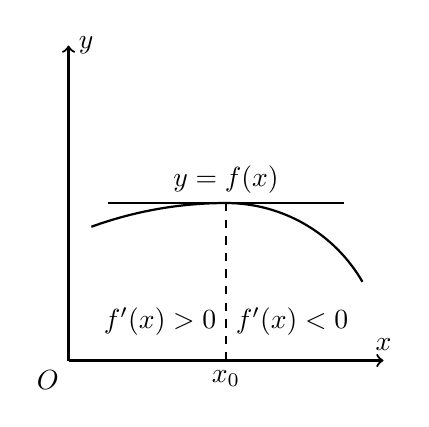
\begin{tikzpicture}
        \draw[thick,->] (0,0) -> (4,0)node[above]{\(x\)};
        \draw[thick,->] (0,0) -> (0,4)node[right]{\(y\)};
        \draw (0,0)node[below left]{\(O\)};
        \draw (2,2)node[above]{\(y=f(x)\)};
        \draw (2,.5)node[left]{\(f'(x)>0\)}node[right]{\(f'(x)<0\)};
        \draw[thick] (2,2)[rotate=90]arc[start angle=0,end angle=-60,radius=2];
        \draw[thick] (2,2)[rotate=90]arc[start angle=0,end angle=20,radius=5];
        \draw (.5,2)--(3.5,2);
        \draw[dashed] (2,2)--(2,0)node[below]{\(x_0\)};
        \end{tikzpicture}
    \subcaption{}
    \end{subfigure}%
    \begin{subfigure}[b]{\subwidth}
    \centering
        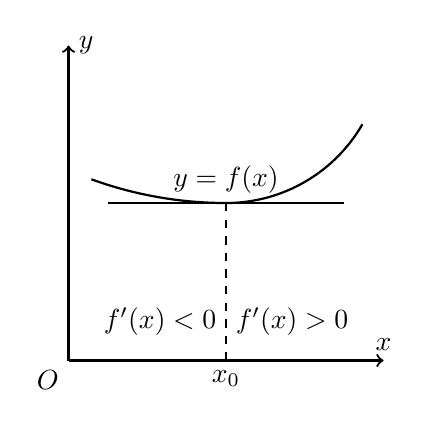
\begin{tikzpicture}
        \draw[thick,->] (0,0) -> (4,0)node[above]{\(x\)};
        \draw[thick,->] (0,0) -> (0,4)node[right]{\(y\)};
        \draw (0,0)node[below left]{\(O\)};
        \draw (2,2)node[above]{\(y=f(x)\)};
        \draw (2,.5)node[left]{\(f'(x)<0\)}node[right]{\(f'(x)>0\)};
        \draw[thick] (2,2)[rotate=-90]arc[start angle=0,end angle=60,radius=2];
        \draw[thick] (2,2)[rotate=-90]arc[start angle=0,end angle=-20,radius=5];
        \draw (.5,2)--(3.5,2);
        \draw[dashed] (2,2)--(2,0)node[below]{\(x_0\)};
        \end{tikzpicture}
    \subcaption{}
    \end{subfigure}%
    \\
    \begin{subfigure}[b]{\subwidth}
    \centering
        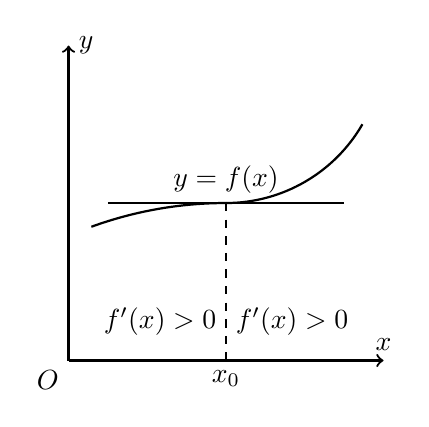
\begin{tikzpicture}
        \draw[thick,->] (0,0) -> (4,0)node[above]{\(x\)};
        \draw[thick,->] (0,0) -> (0,4)node[right]{\(y\)};
        \draw (0,0)node[below left]{\(O\)};
        \draw (2,2)node[above]{\(y=f(x)\)};
        \draw (2,.5)node[left]{\(f'(x)>0\)}node[right]{\(f'(x)>0\)};
        \draw[thick] (2,2)[rotate=-90]arc[start angle=0,end angle=60,radius=2];
        \draw[thick] (2,2)[rotate=90]arc[start angle=0,end angle=20,radius=5];
        \draw (.5,2)--(3.5,2);
        \draw[dashed] (2,2)--(2,0)node[below]{\(x_0\)};
        \end{tikzpicture}
    \subcaption{}
    \end{subfigure}%
    \begin{subfigure}[b]{\subwidth}
    \centering
        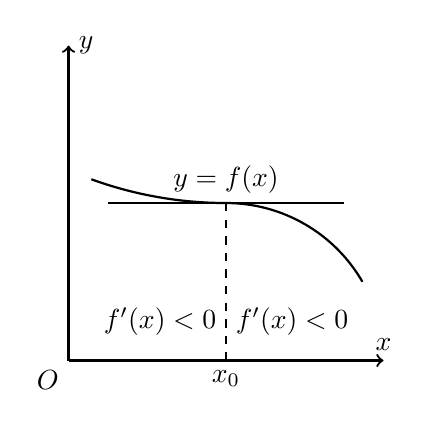
\begin{tikzpicture}
        \draw[thick,->] (0,0) -> (4,0)node[above]{\(x\)};
        \draw[thick,->] (0,0) -> (0,4)node[right]{\(y\)};
        \draw (0,0)node[below left]{\(O\)};
        \draw (2,2)node[above]{\(y=f(x)\)};
        \draw (2,.5)node[left]{\(f'(x)<0\)}node[right]{\(f'(x)<0\)};
        \draw[thick] (2,2)[rotate=90]arc[start angle=0,end angle=-60,radius=2];
        \draw[thick] (2,2)[rotate=-90]arc[start angle=0,end angle=-20,radius=5];
        \draw (.5,2)--(3.5,2);
        \draw[dashed] (2,2)--(2,0)node[below]{\(x_0\)};
        \end{tikzpicture}
    \subcaption{}
    \end{subfigure}%
    \caption{}
    \end{figure}

类似地,可证情形2及情形3.
\end{proof}
\end{theorem}
上述定理也可简单地表述为:当\(x\)在\(x_0\)的邻域内由小及大经过\(x_0\)时,如果\(f'(x)\)的符号由正变负(即\(f'_-(x_0)>0\)且\(f'_+(x_0)<0\)),那么\(f(x)\)在\(x_0\)处取得极大值;如果\(f'(x)\)的符号由负变正(即\(f'_-(x_0)<0\)且\(f'_+(x_0)>0\)),那么\(f(x)\)在\(x_0\)处取得极小值;如果\(f'(x)\)的符号并不改变,那么\(f(x)\)在\(x_0\)处没有极值.

根据上面的两个定理,如果函数\(f(x)\)在所讨论的区间内连续,除个别点歪处处可导,那么就可以按下列步骤来求\(f(x)\)在该区间内的极值点和相应的极值:\begin{enumerate}
\item 求出导数\(f'(x)\);
\item 求出\(f(x)\)的全部驻点与不可导点;
\item 考察\(f'(x)\)的符号在每个驻点或不可导点的左右邻域的情形,以确定该点是否为极值点;如果是极值点,进一步确定是极大值点还是极小值点;
\item 求出各极值点的函数值,就得函数\(f(x)\)的全部极值.
\end{enumerate}

\begin{theorem}[函数存在极值的第二充分条件]\label{theorem:微分中值定理.函数存在极值的第二充分条件}
设函数\(f(x)\)在\(x_0\)处具有二阶导数且\(f'(x_0)=0\),\(f''(x_0)\neq 0\),那么
\begin{enumerate}
\item 当\(f''(x_0)<0\)时,函数\(f(x)\)在\(x_0\)处取得极大值;
\item 当\(f''(x_0)>0\)时,函数\(f(x)\)在\(x_0\)处取得极小值.
\end{enumerate}
\end{theorem}
上述定理表明,如果函数\(f(x)\)在驻点\(x_0\)处的二阶导数\(f''(x_0)\neq0\),那么该驻点\(x_0\)一定是极值点,并且可以按二阶导数\(f''(x_0)\)的符号来判定\(f(x_0)\)是极大值还是极小值.但如果\(f''(x_0)=0\),上述定理就不能应用.事实上,当\(f'(x_0)=0\)且\(f''(x_0)=0\)时,\(f(x)\)在\(x_0\)处可能有极大值,也可能有极小值,也可能没有极值;例如,\(f_1(x) = -x^4\),\(f_2(x) = x^4\)和\(f_3(x) = x^3\)这三个函数在\(x=0\)处就分别属于这三种情况.因此,如果函数在驻点处的二阶导数为零,那么还得用一阶导数在驻点左右邻域的符号来判定.

\begin{example}
设函数\(f(x),g(x)\)都具有二阶导数,且\(g''(x)<0\),\(g(x_0)=a\)是\(g(x)\)的极值,证明:“\(f'(a)>0\)”是“\(f[g(x)]\)在\(x_0\)取极大值”的充分条件.
\begin{solution}
因为\(g(x_0)=a\)是\(g(x)\)的极值,所以根据\cref{theorem:微分中值定理.函数存在极值的必要条件} 必有\(g'(x_0)=0\).

记\(F(x) = f[g(x)]\),则\(F'(x) = \eval{f'(u)}_{u=g(x)} \cdot g'(x)\),\(F''(x) = \eval{f''(u)}_{u=g(x)} \cdot g'(x) \cdot g'(x) + \eval{f'(u)}_{u=g(x)} \cdot g''(x)\).
根据\cref{theorem:微分中值定理.函数存在极值的第二充分条件},要使“\(F(x)=f[g(x)]\)在\(x_0\)取极大值”,只需令\(F''(x_0) < 0\),那么有\[
\eval{f'(u_0)}_{u_0=g(x_0)} \cdot g''(x_0) < 0.
\]由题可知\(g''(x)<0\),故\(\eval{f'(u_0)}_{u_0=g(x_0)} = f'(a) > 0\),也就是说“\(f'(a)>0\)”是“\(f[g(x)]\)在\(x_0\)取极大值”的充分条件.
\end{solution}
\end{example}

\subsection{最大值最小值问题}
假定函数\(f(x)\)在闭区间\([a,b]\)上连续,在开区间\((a,b)\)内除有限个点外可导,且至多有有限个驻点.在上述条件下,我们来讨论\(f(x)\)在\([a,b]\)上的最大值和最小值的求法.

首先由闭区间上连续函数的性质,可知\(f(x)\)在\([a,b]\)上的最大值和最小值一定存在.

其次,如果最大值(或最小值)\(f(x_0)\)在开区间\((a,b)\)内的点\(x_0\)处取得,那么,按\(f(x)\)在开区间内除有限个点外可导且至多有有限个驻点的假定,可知\(f(x_0)\)一定也是\(f(x)\)的极大值(或极小值),从而\(x_0\)一定是\(f(x)\)的驻点或不可导点.又\(f(x)\)的最大值和最小值也可能在区间的端点处取得.因此,可用如下的方法求\(f(x)\)在\([a,b]\)上的最大值和最小值.

\begin{enumerate}
\item 求出\(f(x)\)在\((a,b)\)内的驻点\(\AutoTuple{x}{m}\)和不可导点\(x'_1,x'_2,\dotsc,x'_n\);
\item 计算\(f(x_i)\)(\(i=1,2,\dotsc,m\))和\(f(x'_j)\)(\(j=1,2,\dotsc,n\)),以及\(f(a)\)和\(f(b)\);
\item 比较上一步中求出的各个函数值,其中最大的就是\(f(x)\)在\([a,b]\)上的最大值,最小的就是\(f(x)\)在\([a,b]\)上的最小值.
\end{enumerate}

在求函数的最大值(或最小值)时,特别值得指出的是下述情形:\(f(x)\)在一个区间(不论有限区间还是无限区间,开区间或闭区间)内可导,且只有一个驻点\(x_0\),并且这个驻点\(x_0\)是函数\(f(x)\)的极值点,那么,当\(f(x_0)\)是极大值时,\(f(x_0)\)就是\(f(x)\)在该区间上的最大值;当\(f(x_0)\)是极小值时,\(f(x_0)\)就是\(f(x)\)在该区间上的最小值.

\section{函数图形的描绘}
借助一阶导数的符号,可以确定函数图形在哪个区间上上升,在哪个区间上下降,在什么地方有极值点;借助二阶导数的符号,可以确定函数图形在哪个区间上为凹,在哪个区间上为凸,在什么地方有拐点.知道了函数图形的升降、凹凸以及极值点和拐点后,也就可以掌握函数的性态,并把函数的图形画得比较准确.

现在,随着现代计算机技术的发展,借助计算机和许多数学软件,可以方便地画出各种函数的图形.但是,如何识别机器作图中的误差,如何掌握图形上的关键点,如何选择作图的范围等,从而进行人工干预,仍然需要我们有运用微分学的方法描绘图形的基本知识.

利用导数描绘函数图形的一般步骤如下:\begin{enumerate}
\item 确定函数\(y=f(x)\)的定义域及函数所具有的某些特性(如奇偶性、周期性等),并求出函数的一阶导数\(f'(x)\)和二阶导数\(f''(x)\);
\item 求出一阶导数\(f'(x)\)和二阶导数\(f''(x)\)在函数定义域内的全部零点,并求出函数\(f(x)\)的间断点及\(f'(x)\)和\(f''(x)\)不存在的点,用这些点把函数的定义域划分成几个部分区间;
\item 确定在这些部分区间内\(f'(x)\)和\(f''(x)\)的符号,并由此确定函数图形的升降、凹凸、极值点、拐点;
\item 确定函数图形的水平渐近线、铅直渐近线、斜渐近线以及其他变化趋势;
\item 算出\(f'(x)\)和\(f''(x)\)的零点以及不存在的点所对应的函数值,定出图形上的相应的点;为了把图形描绘得准确些,有时还需要补充一些点;然后结合前两步中得到的结果,联结这些点画出函数\(y=f(x)\)的图形.
\end{enumerate}

\section{曲率}\label{section:微分中值定理.曲率}
\subsection{弧微分}
作为曲率的预备知识,先介绍弧微分的概念.

设函数\(f(x)\)在区间\((a,b)\)内具有连续导数.在曲线\(y=f(x)\)上取固定点\(M_0\opair{x_0,y_0}\)作为度量弧长的基点,并规定依\(x\)增大的方向作为曲线的正向.对曲线上任一点\(M\opair{x,y}\),规定有向弧段\(\arc{M_0 M}\)的值\(s\)(简称为弧\(s\))如下:\(s\)的绝对值等于这弧段的长度,当有向弧段\(\arc{M_0 M}\)的方向与曲线的正向一致时\(s>0\),相反时\(s<0\).显然,弧\(s\)与\(x\)存在函数关系:\(s = s(x)\),而且\(s(x)\)是\(x\)的单调增加函数.下面来求\(s(x)\)的导数及微分.

设\(x\)、\(x+\increment x\)为\((a,b)\)内两个邻近的点,它们在曲线\(y=f(x)\)上的对应点为\(M\)、\(M'\),并设对应于\(x\)的增量\(\increment x\),弧\(s\)的增量为\(\increment s\),那么\[
\increment s = \arc{M_0 M'} - \arc{M_0 M} = \arc{M M'}.
\]于是\begin{align*}
\left(\frac{\increment s}{\increment x}\right)^2
&= \left(\frac{\arc{M M'}}{\increment x}\right)^2
= \left(\frac{\arc{M M'}}{\abs{M M'}}\right)^2 \cdot \frac{\abs{M M'}^2}{(\increment x)^2} \\
&= \left(\frac{\arc{M M'}}{\abs{M M'}}\right)^2 \cdot \frac{(\increment x)^2 + (\increment y)^2}{(\increment x)^2} \\
&= \left(\frac{\arc{M M'}}{\abs{M M'}}\right)^2 \cdot \left[ 1 + \left(\frac{\increment y}{\increment x}\right)^2 \right],
\end{align*}\[
\frac{\increment s}{\increment x} = \pm \sqrt{\left(\frac{\arc{M M'}}{\abs{M M'}}\right)^2 \cdot \left[ 1 + \left(\frac{\increment y}{\increment x}\right)^2 \right]}.
\]令\(\increment x\to0\)取极限,由于\(\increment x\to0\)时,\(M' \to M\),这时弧的长度与弦的长度之比的极限等于1,即\[
\lim\limits_{M' \to M} \frac{\abs{\arc{M M'}}}{\abs{M M'}} = 1,
\]又\[
\lim\limits_{\increment x\to0} \frac{\increment y}{\increment x} = y',
\]因此得\[
\dv{s}{s} = \pm \sqrt{1 + y'^2}.
\]由于\(s = s(x)\)是单调增加函数,从而上式根号前应取正号,即\begin{equation}
\dd{s} = \sqrt{1 + y'^2} \dd{x},
\end{equation}这就是\DefineConcept{弧微分公式}.

弧微分公式也可写作\begin{equation}
\dd{s} = \sqrt{(\dd{x})^2 + (\dd{y})^2}.
\end{equation}

\subsection{曲率及其计算公式}
设曲线\(C\)是光滑的(即曲线上每一点处都具有切线,且切线随切点的移动而连续转动),在曲线\(C\)上选定一点\(M_0\)作为度量弧\(s\)的基点.设曲线上点\(M\)对应于弧\(s\),在点\(M\)处切线的倾角为\(\alpha\)(这里假定曲线\(C\)所在的平面上已设立了\(xOy\)坐标系),曲线上另外一点\(M'\)对应于弧\(s+\increment s\),在点\(M'\)处切线的倾角为\(\alpha + \increment \alpha\).那么,弧段\(\arc{MM'}\)的长度为\(\abs{\increment s}\).
当动点从\(M\)移动到\(M'\)时切线转过的角度为\(\abs{\increment \alpha}\).

我们用比值\(\frac{\abs{\increment\alpha}}{\abs{\increment s}}\),即单位弧段上切线转过的角度的大小来表达弧段\(\arc{MM'}\)的平均弯曲程度,把这比值叫做弧段\(\arc{MM'}\)的\DefineConcept{平均曲率},并记作\(\overline{K}\),即\[
\overline{K} = \abs{\frac{\increment\alpha}{\increment s}}.
\]

类似于从平均速度引进瞬时速度的方法,当\(\increment s\to0\)(即\(M' \to M\))时,上述平均曲率的极限叫做曲线\(C\)在点\(M\)处的\DefineConcept{曲率},记作\(K\),即\[
K = \lim\limits_{\increment s\to0} \abs{\frac{\increment\alpha}{\increment s}}.
\]在\(\displaystyle \lim\limits_{\increment s\to0} \frac{\increment\alpha}{\increment s} = \dv{\alpha}{s}\)存在的条件下,\(K\)也可以表示为\[
K = \abs{\dv{\alpha}{s}}.
\]

对于直线来说,切线与直线本身重合,当点沿直线移动时,切线的倾角不变,\(\increment\alpha = 0\),\(\frac{\increment\alpha}{\increment s} = 0\),从而\(K = \abs{\displaystyle\dv{\alpha}{s}} = 0\).这就是说,直线上任意点\(M\)处的曲率都等于零,这与我们直觉认识到的“直线不弯曲”一致.

\begin{figure}%曲率圆
\centering
\begin{tikzpicture}
\draw[thick,->] (0,0) -> (9,0)node[above]{\(x\)};
\draw[thick,->] (0,0) -> (0,8)node[right]{\(y\)};
\pgfmathsetmacro{\cx}{4}
\pgfmathsetmacro{\cy}{4}
\pgfmathsetmacro{\cr}{3}
\coordinate(M)at(\cx,\cy);
\draw (M)circle(\cr);
\pgfmathsetmacro{\ta}{30}
\pgfmathsetmacro{\tb}{80}
\pgfmathsetmacro{\pax}{\cx+\cr*sin(\ta)}
\pgfmathsetmacro{\pay}{\cy-\cr*cos(\ta)}
\pgfmathsetmacro{\pbx}{\cx+\cr*sin(\tb)}
\pgfmathsetmacro{\pby}{\cy-\cr*cos(\tb)}
\coordinate(P1)at(\pax,\pay);
\coordinate(P2)at(\pbx,\pby);
\draw (M)node[left]{\(D\)}--(P1)node[below]{\(M\)}
	(M)--(P2)node[right]{\(M'\)}node[midway,above]{\(a\)};
\pgfmathsetmacro{\paz}{\pax+\pay*(\cy-\pay)/(\cx-\pax)}
\pgfmathsetmacro{\pbz}{\pbx+\pby*(\cy-\pby)/(\cx-\pbx)}
\coordinate(Q1)at(\paz,0);
\coordinate(Q2)at(\pbz,0);
\coordinate(X)at(100,0);
\draw (Q1)--(P1) (Q2)--(P2);

\draw pic["\(\increment\alpha\)",draw=orange,-,below right]{angle=P1--M--P2};
\draw pic["\(\alpha\)",draw=orange,-,angle eccentricity=1.5,angle radius=5mm]{angle=X--Q1--P1};
\draw pic["\(\alpha+\increment\alpha\)",draw=orange,-,angle eccentricity=1,angle radius=3mm,above right]{angle=X--Q2--P2};
\draw pic[draw=gray,-,angle radius=0.3cm]{right angle=M--P1--Q1};
\draw pic[draw=gray,-,angle radius=0.3cm]{right angle=M--P2--Q2};
\end{tikzpicture}
\caption{曲率圆}
\label{figure:微分中值定理.曲率圆}
\end{figure}

设圆的半径为\(a\),由\cref{figure:微分中值定理.曲率圆} 可见,圆在点\(M\)、\(M'\)处的切线所夹的角\(\increment\alpha\)等于中心角\(\angle{M D M'}\).但\(\angle{M D M'} = \frac{\increment s}{a}\),于是\[
\frac{\increment\alpha}{\increment s} = \frac{\increment s / a}{\increment s} = \frac{1}{a},
\]从而\[
K = \abs{\dv{\alpha}{s}} = \frac{1}{a}.
\]因为点\(M\)是圆上任意取定的一点,上述结论表示圆上各点处的曲率都等于半径\(a\)的倒数\(\frac{1}{a}\),这就是说,圆的弯曲程度到处一样,且半径越小曲率越大,即圆弯曲得越厉害.

设曲线的直角坐标方程为\(y=f(x)\),且\(f(x)\)具有二阶导数(这时\(f'(x)\)连续,从而曲线是光滑的).因为\(\tan\alpha = y'\),所以\[
\sec^2\alpha \dv{\alpha}{x} = y'',
\]\[
\dv{\alpha}{x} = \frac{y''}{1 + \tan^2\alpha} = \frac{y''}{1 + y'^2},
\]于是\[
\dd{\alpha} = \frac{y''}{1 + y'^2} \dd{x}.
\]又因为\(\dd{s} = \sqrt{1+y'^2} \dd{x}\),从而有\begin{equation}
K = \frac{\abs{y''}}{(1+y'^2)^{3/2}}.
\end{equation}

设曲线由参数方程\(\left\{ \begin{array}{c} x = \varphi(t) \\ y = \psi(t) \end{array} \right.\)给出,那么有\begin{equation}
K = \frac{\abs{\varphi'(t)\psi''(t)-\varphi''(t)\psi'(t)}}{[\varphi'^2(t)+\psi'^2(t)]^{3/2}}.
\end{equation}

在某些实际问题中,\(\abs{y'}\)同\(1\)比较起来是很小的(即\(\abs{y'} \ll 1\)),可以忽略不计,这时,由\(1 + y'^2 \approx 1\),而有曲率的近似计算公式为\[
K \approx \abs{y''}.
\]这就是说,当\(\abs{y'} \ll 1\)时,曲率\(K\)近似于\(\abs{y''}\).经过这样的简化之后,对一些复杂问题的计算和讨论就方便多了.

\subsection{曲率圆与曲率半径}
设曲线\(y=f(x)\)在点\(M\opair{x,y}\)处的曲率为\(K\)(\(K\neq0\)).在点\(M\)处的曲线的发现上,在凹的一侧取一点\(D\),使\(\abs{DM} = \frac{1}{K} = \rho\).以\(D\)为圆心,\(\rho\)为半径作圆,这个圆叫做曲线在点\(M\)处的\DefineConcept{曲率圆},曲率圆的圆心\(D\)叫做曲线在点\(M\)处的\DefineConcept{曲率中心},曲率圆的半径\(\rho\)叫做曲线在点\(M\)处的\DefineConcept{曲率半径}.

按上述规定可知,曲率圆与曲线在点\(M\)有相同的切线和曲率,且在点\(M\)邻近有相同的凹向.因此,在实际问题中,常常用曲率圆在点\(M\)邻近的一段圆弧来近似代替曲线弧,以使问题简化.

按上述规定,曲线在点\(M\)处的曲率\(K\)(\(K\neq0\))与曲线在点\(M\)处的曲率半径\(\rho\)有如下的关系:\[
\rho = \frac{1}{K}, \qquad K = \frac{1}{\rho}.
\]这就是说:曲线上一点处的曲率半径与曲线在该点处的曲率互为倒数.

\begin{example}
求出对数曲线\(y = \ln x\)上曲率半径最小的点.
\begin{solution}
显然有\(y' = \frac{1}{x}\),\(y'' = -\frac{1}{x^2}\),那么曲率为\[
K = \frac{\abs{y''}}{(1+y'^2)^{3/2}}
= \frac{1/x^2}{(1+1/x^2)^{3/2}}
= \frac{x}{(1+x^2)^{3/2}}.
\]曲率\(K\)对\(x\)求导得\[
K' = \frac{(1+x^2)^{3/2} - x \frac{3}{2} (1+x^2)^{1/2} 2x}{(1+x^2)^3}
= \frac{1 - 2x^2}{(1+x^2)^{5/2}}.
\]令\(K' = 0\),考虑\(x>0\),解得\(x_0 = \frac{1}{\sqrt{2}}\).当\(0<x<x_0\)时,\(K'>0\);当\(x>x_0\)时,\(K'<0\);说明\(K'\)在\(x=x_0\)时取得极大值.而曲率半径最小的点就是曲率最大的点,即\(x = \frac{1}{\sqrt{2}}\)时,曲率半径最小值为\(\frac{3\sqrt{3}}{2}\).
\end{solution}
\end{example}

\subsection{曲率中心的计算公式以及渐屈线、渐伸线}
设已知曲线的方程是\(y=f(x)\),且其二阶导数\(y''\)在点\(x\)不为零,则曲线在对应点\(M\opair{x,y}\)的曲率中心\(D\opair{\alpha,\beta}\)的坐标为\begin{equation}
\left\{ \def\arraystretch{1.5} \begin{array}{l}
\alpha = x - y' \frac{1 + y'^2}{y''}, \\
\beta = y + \frac{1 + y'^2}{y''}.
\end{array} \right.
\end{equation}

当点\(\opair{x,f(x)}\)沿曲线\(C\)移动时,相应的曲率中心\(D\)的轨迹曲线\(G\)称为曲线\(C\)的\DefineConcept{渐屈线},相对地,曲线\(C\)称为曲线\(G\)的\DefineConcept{渐伸线}.
